\chapter{Introduction}
\minitoc
\label{Cap:Int}
%%%%%%%%%%%%%%%%%%%%%%%%%%%%%%%%%%%%%%%%%%%%%%%%%%
% 
\section{Standard Model}
The Standard Model of Particles (SM) is a unified quantum field theory of the electroweak interaction and Quantum Chromodynamics (QCD). It models fundamental objects, quantum fields, that represents 17 fundamental particles, with their respective antiparticles.

The elementary particles are divides in two meanly blocks: 
\begin{itemize}
    \item The fermions, these particles are commonly know as the matter particles (or antimatter particles). These are fractional spin particles and are divides in two mainly blocks, quarks and leptons. These are described in more depth later. 
    \item The bosons, these particles are the carriers of the weak, strong and electromagnetic fundamental interactions. The Higgs field, it is a field that supplement the SM by the Higgs mechanism to generate masses to the bosons and fermions. These are described in more depth later.
\end{itemize}

The agreement of the SM predictions with most precise measurements of the particle experiments, provides a high confidence in this model. However, it is not complete, there are phenomena that are not described by it, such as the case of dark mater and neutrino oscillations.

\begin{figure}[!htb]
\centering
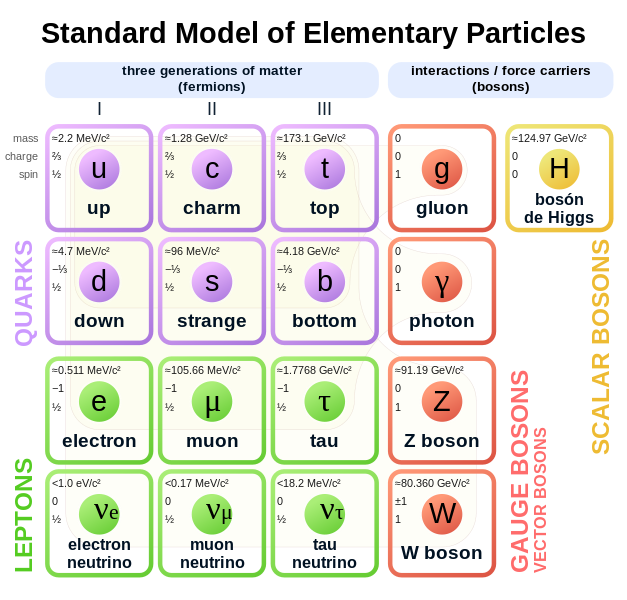
\includegraphics[scale=0.5]{Figures/Chapter1/Standard_Model_of_Elementary_Particles.png}

        \caption{In the figure is shown a pictorial summary of the standard model. In this are shown the the 17 particles of the SM. Something that should be considered is that there are other 17 that correspond to the antiparticle of each particle. Figure from \cite{SM_Table}} 
\label{fig:SM}
\end{figure}
 
\subsection{Bosons}
Bosons and fermions are differentiated by their spin characteristics. Bosons have integer values for spin, while fermions have half-integer values. In the SM, the elementary particles interacts through the gauge bosons, which acts as carriers for the fundamental forces of weak, strong and electromagnetic interactions. The Higgs boson plays a crucial role in the Higgs Mechanism, whereby particles gain mass through their interaction with this boson. Additionally, there is a hypothetical boson called as graviton, this particle should be the carrier of the gravitational force, it have no been observed yet \textbf{Agregar bibliografia}.  

\subsubsection{The electromagnetic force}
Described by the quantum electrodynamics, the electromagnetic force is transmitted by photons, which interact exclusively with charged spin 1/2 particles. The mass of the photons is 0. This force is capable of acting over long distances. These are the responsible of  The effects of electromagnetic force are observable on a macroscopic scale, and it finds numerous practical applications.

\subsubsection{Strong Force}
It is carried by the gluons, these are the responsible to joint quarks and generate hadrons. This force is also the responsible to joint the neutrons and protons in the interior of the atomic nucleus. The interactions mediated by strong force are modeled by the Quantum Chromodynamics (QCD). Here the charge is represented as "color", which is carried only by quarks.

In QCD, There are three color charges (red, blue and green). The quarks has one charge color and the gluons are has two colors. In the strong interactions the color of thee quarks may change but as the same with the electric charge the color is always conserved. Unlike photons, the gluons are capable to interact with other gluons this make more complicated the consider all the interactions that    
 

\subsubsection{The weak force}
It is carried by the bosons $W^\pm$ and $Z$. This force is the responsible of various particles decays and in some scattering processes. All the elementary fermions may interacts by this force, in the case of the neutrinos it is the only known way that this particle interacts.

There are two types of interactions, the Charge Current (CC) interaction an the Neutral Current (NC) interaction. The CC interactions occurs when particles interacts by the $W^\pm$ boson, In this tipe of interaction 

\subsection{Fermions}
These are the blocks of the matter, 12 of the 17 fundamental particles are Fermions, these are defined as particles with half integer spin. These are divided in quarks and  leptons. 

\textbf{Quarks}
The quarks are described by the QCD, it is a gauge theory based on SU(3) symmetry.  

\textbf{Leptons}
In the SM are 6 different leptons known, with their respective antiparticles. These are divided in 3 groups called generations, these can be represented doublets: 

$\begin{pmatrix}
    \nu_e \\
    e^-
\end{pmatrix}$, 
$\begin{pmatrix}
    \nu_\mu \\
    \mu^-
\end{pmatrix}$, 
$\begin{pmatrix}
    \nu_\tau \\
    \tau^-
\end{pmatrix}$

The electron $e^-$, muon $\mu^-$ and tau $\tau^-$ are electrical charged leptons; with a charge $-e$, were $e$ is the magnitude of charge of the electron , these leptons interact by electromagnetic and weak forces. 

The $\nu_e$, $\nu_\mu$ and $\nu_\tau$ are electrical neutral leptons, this only interacts by weak force. These leptons are known as neutrinos and depend the generation these are called electron-neutrino ($\nu_e$), muon-neutrino ($\nu_\mu$) or tau-neutrino. 

\subsection{Neutrinos}
The neutrinos are the most abundant particles with mass in the universe of the SM. These are leptons, with out electrical charge. 

\subsubsection{Brief story of the neutrinos}
During the beginning of last century, the nuclear physicist studied the radioactivity of different materials. During this studies the identify meanly 3 types of nuclear decays: $\alpha$-decay, $\beta$-decay and the $\gamma$-decay. The energy of the  $\alpha$-decay and $\gamma$-decay is discrete and depend of the atomic nucleus that emits the radiation. The spectrum energy shows characteristic picks for certainly values of energy, in the \textbf{Figure} \ref{fig:abgSpectrum} two examples of energy spectrum for alpha and gamma emissions are shown. On the other hand, the $\beta$-decay processes produce a continuum spectra, in the \textbf{Figure} \ref{fig:abgSpectrum}an example of $\beta$-decay energy spectrum is shown. The fact that the energy spectrum of the $\beta$-decay electron is a continuum represents that a portion of the energy were lost or a violation of the energy conservation law.

\begin{figure}[!htb]
\centering
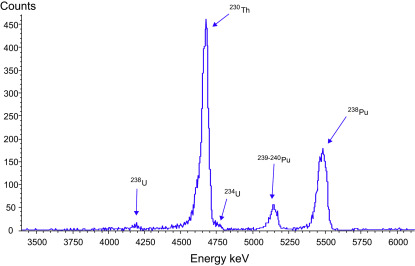
\includegraphics[scale=0.8]{Figures/Chapter1/alphaspectrum.jpg}
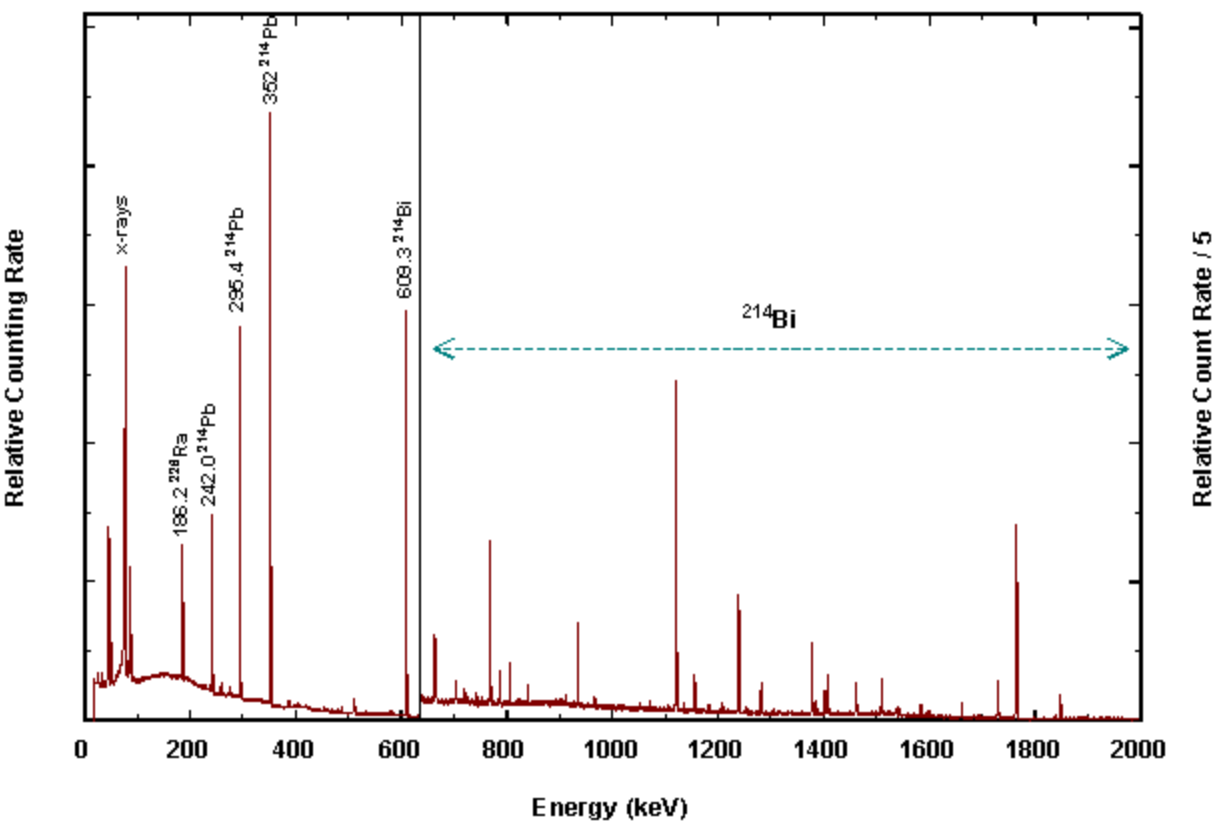
\includegraphics[scale=0.2]{Figures/Chapter1/radspec_gamma.png}
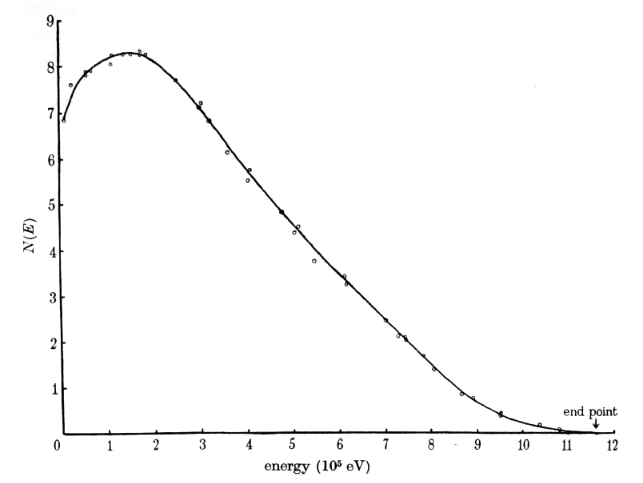
\includegraphics[scale=0.25]{Figures/Chapter1/Ra_betaSpec.png}

        \caption{Top plot, alpha spectrum of mixture of radioactive materials measured by a gas detector\cite{alphaSpectrum}. Middle plot, gamma spectrum of Radium-226 from high purity germanium detector\cite{RaSpectrum_gamma}. Bottom plot, spectrum of energy of electron from beta decay in of Ra\cite{Ra_betaSpec}} 
\label{fig:abgSpectrum}
\end{figure}

In 1930 Wolfgang Pauli \cite{NeutrinoHistory} proposed in a letter that the continuum spectra might be due to one more "invisible" light neutral particle, this should have spin 1/2 and obey the exclusion principle, he call this particle \textit{neutrons}. In the letter Pauli explain that with this particle the electron would be able to take any momentum until the maximum limit allowed ant the other particle has the residual momentum. In 1932 Chadwick discovered the neutron, it did not match with the Pauli description. In 1933, Enrico Fermi adopted the name of \textit{neutrino} for the particle proposed by Pauli; Fermi propoused a model where the neutrino should be a $^1/_2$ spin particle (a fermion). In 1953 the neutrinos were observed by the experiment of Clyde Cowan and Frederick Reines \textcolor{red}{Agregar referencia del descubrimiento del neutrino}. In this experiment they measured the anti-neutrinos produced in Savanna River Reactor in South Carolina and they show that .




 

